%%%%%%%%%%%%%%%%%%%%%%%%%%%%%%%%%%%%%%%%%%%%%%%%%%%%%%%%%%%%%%%%%%%%
%% I, the copyright holder of this work, release this work into the
%% public domain. This applies worldwide. In some countries this may
%% not be legally possible; if so: I grant anyone the right to use
%% this work for any purpose, without any conditions, unless such
%% conditions are required by law.
%%%%%%%%%%%%%%%%%%%%%%%%%%%%%%%%%%%%%%%%%%%%%%%%%%%%%%%%%%%%%%%%%%%%

\documentclass[
  digital, %% This option enables the default options for the
           %% digital version of a document. Replace with `printed`
           %% to enable the default options for the printed version
           %% of a document.
  table,   %% Causes the coloring of tables. Replace with `notable`
           %% to restore plain tables.
  nolof,     %% Prints the List of Figures. Replace with `nolof` to
           %% hide the List of Figures.
  nolot,     %% Prints the List of Tables. Replace with `nolot` to
           %% hide the List of Tables.
  %% More options are listed in the user guide at
  %% <http://mirrors.ctan.org/macros/latex/contrib/fithesis/guide/mu/fi.pdf>.
]{fithesis3}
%% The following section sets up the locales used in the thesis.
\usepackage[resetfonts]{cmap} %% We need to load the T2A font encoding
\usepackage[T1,T2A]{fontenc}  %% to use the Cyrillic fonts with Russian texts.
\usepackage[
  main=english, %% By using `czech` or `slovak` as the main locale
                %% instead of `english`, you can typeset the thesis
                %% in either Czech or Slovak, respectively.
  german, russian, czech, slovak %% The additional keys allow
]{babel}        %% foreign texts to be typeset as follows:
%%
%%   \begin{otherlanguage}{german}  ... \end{otherlanguage}
%%   \begin{otherlanguage}{russian} ... \end{otherlanguage}
%%   \begin{otherlanguage}{czech}   ... \end{otherlanguage}
%%   \begin{otherlanguage}{slovak}  ... \end{otherlanguage}
%%
%% For non-Latin scripts, it may be necessary to load additional
%% fonts:
\usepackage{paratype}
\def\textrussian#1{{\usefont{T2A}{PTSerif-TLF}{m}{rm}#1}}
%%
%% The following section sets up the metadata of the thesis.
\thesissetup{
    date          = 2017/01/04,
    university    = mu,
    faculty       = fi,
    type          = mgr,
    author        = Bc. David Kouřil,
    gender        = m,
    advisor       = Mathieu Le Muzic and Ivan Viola and Barbora Kozlikova,
    title         = {Maya2CellVIEW: Integrated Tool for Creating Large and Complex Molecular Scenes},
    TeXtitle      = {Maya2CellVIEW: Integrated Tool for Creating Large and Complex Molecular Scenes},
    keywords      = {molecular visualization, illustration, Maya, Unity, ...},
    TeXkeywords   = {keyword1, keyword2, \ldots},
    bib           = example.bib,
}
\thesislong{abstract}{
    Scientific illustrators communicate the cutting edge of research through their illustrations. There are numerous software tools that assist them with this job. The aim of this thesis is to push abilities of illustrators working on a large scale molecular scenes. This is done by connecting two software packages - Maya and cellVIEW - combining the rendering possibilities of cellVIEW and modeling tools of Maya which results in more effective and efficient workflow. 
}
\thesislong{thanks}{
    This is the acknowledgement for my thesis, which can

    span multiple paragraphs.
}
%% The following section sets up the bibliography.
\usepackage{csquotes}
\usepackage[              %% When typesetting the bibliography, the
 backend=biber,          %% `numeric` style will be used for the
%  backend=bibtex,
  style=numeric,          %% entries and the `numeric-comp` style
  citestyle=numeric-comp, %% for the references to the entries. The
  sorting=none,           %% entries will be sorted in cite order.
  sortlocale=auto         %% For more unformation about the available
]{biblatex}               %% `style`s and `citestyles`, see:
%% <http://mirrors.ctan.org/macros/latex/contrib/biblatex/doc/biblatex.pdf>.
\addbibresource{example.bib} %% The bibliograpic database within
                          %% the file `example.bib` will be used.
\usepackage{makeidx}      %% The `makeidx` package contains
\makeindex                %% helper commands for index typesetting.
%% These additional packages are used within the document:
\usepackage{paralist}
\usepackage{amsmath}
\usepackage{amsthm}
\usepackage{amsfonts}
\usepackage{url}
\usepackage{menukeys}
\begin{document}
\chapter{Introduction}
\label{chap:introduction}
%[\textbf{In what field are we? What are the people in this domain doing?}]
In this day and age, scientists come to new findings every day. Unfortunately, not all of these are ever shown to the general public. There can be several reasons for that. New discovered facts are usually pieces of a bigger picture. Also, all the information might be already there, in several databases, but putting it all together would take significant effort and time.
On top of that, scientists are not usually trained to expose their results to the public eye.

This is the job of scientific illustrator. These people are, first and foremost, experts in their fields but on top of that they have invested significant amount of time on acquiring and perfecting their artistic skills. They use these skills to visualize the science in their domain with easily understandable images, animations or other forms of media. %if somebody asks - ex. arthur olson 3d prints and sculptures
\begin{figure}
  \centering
  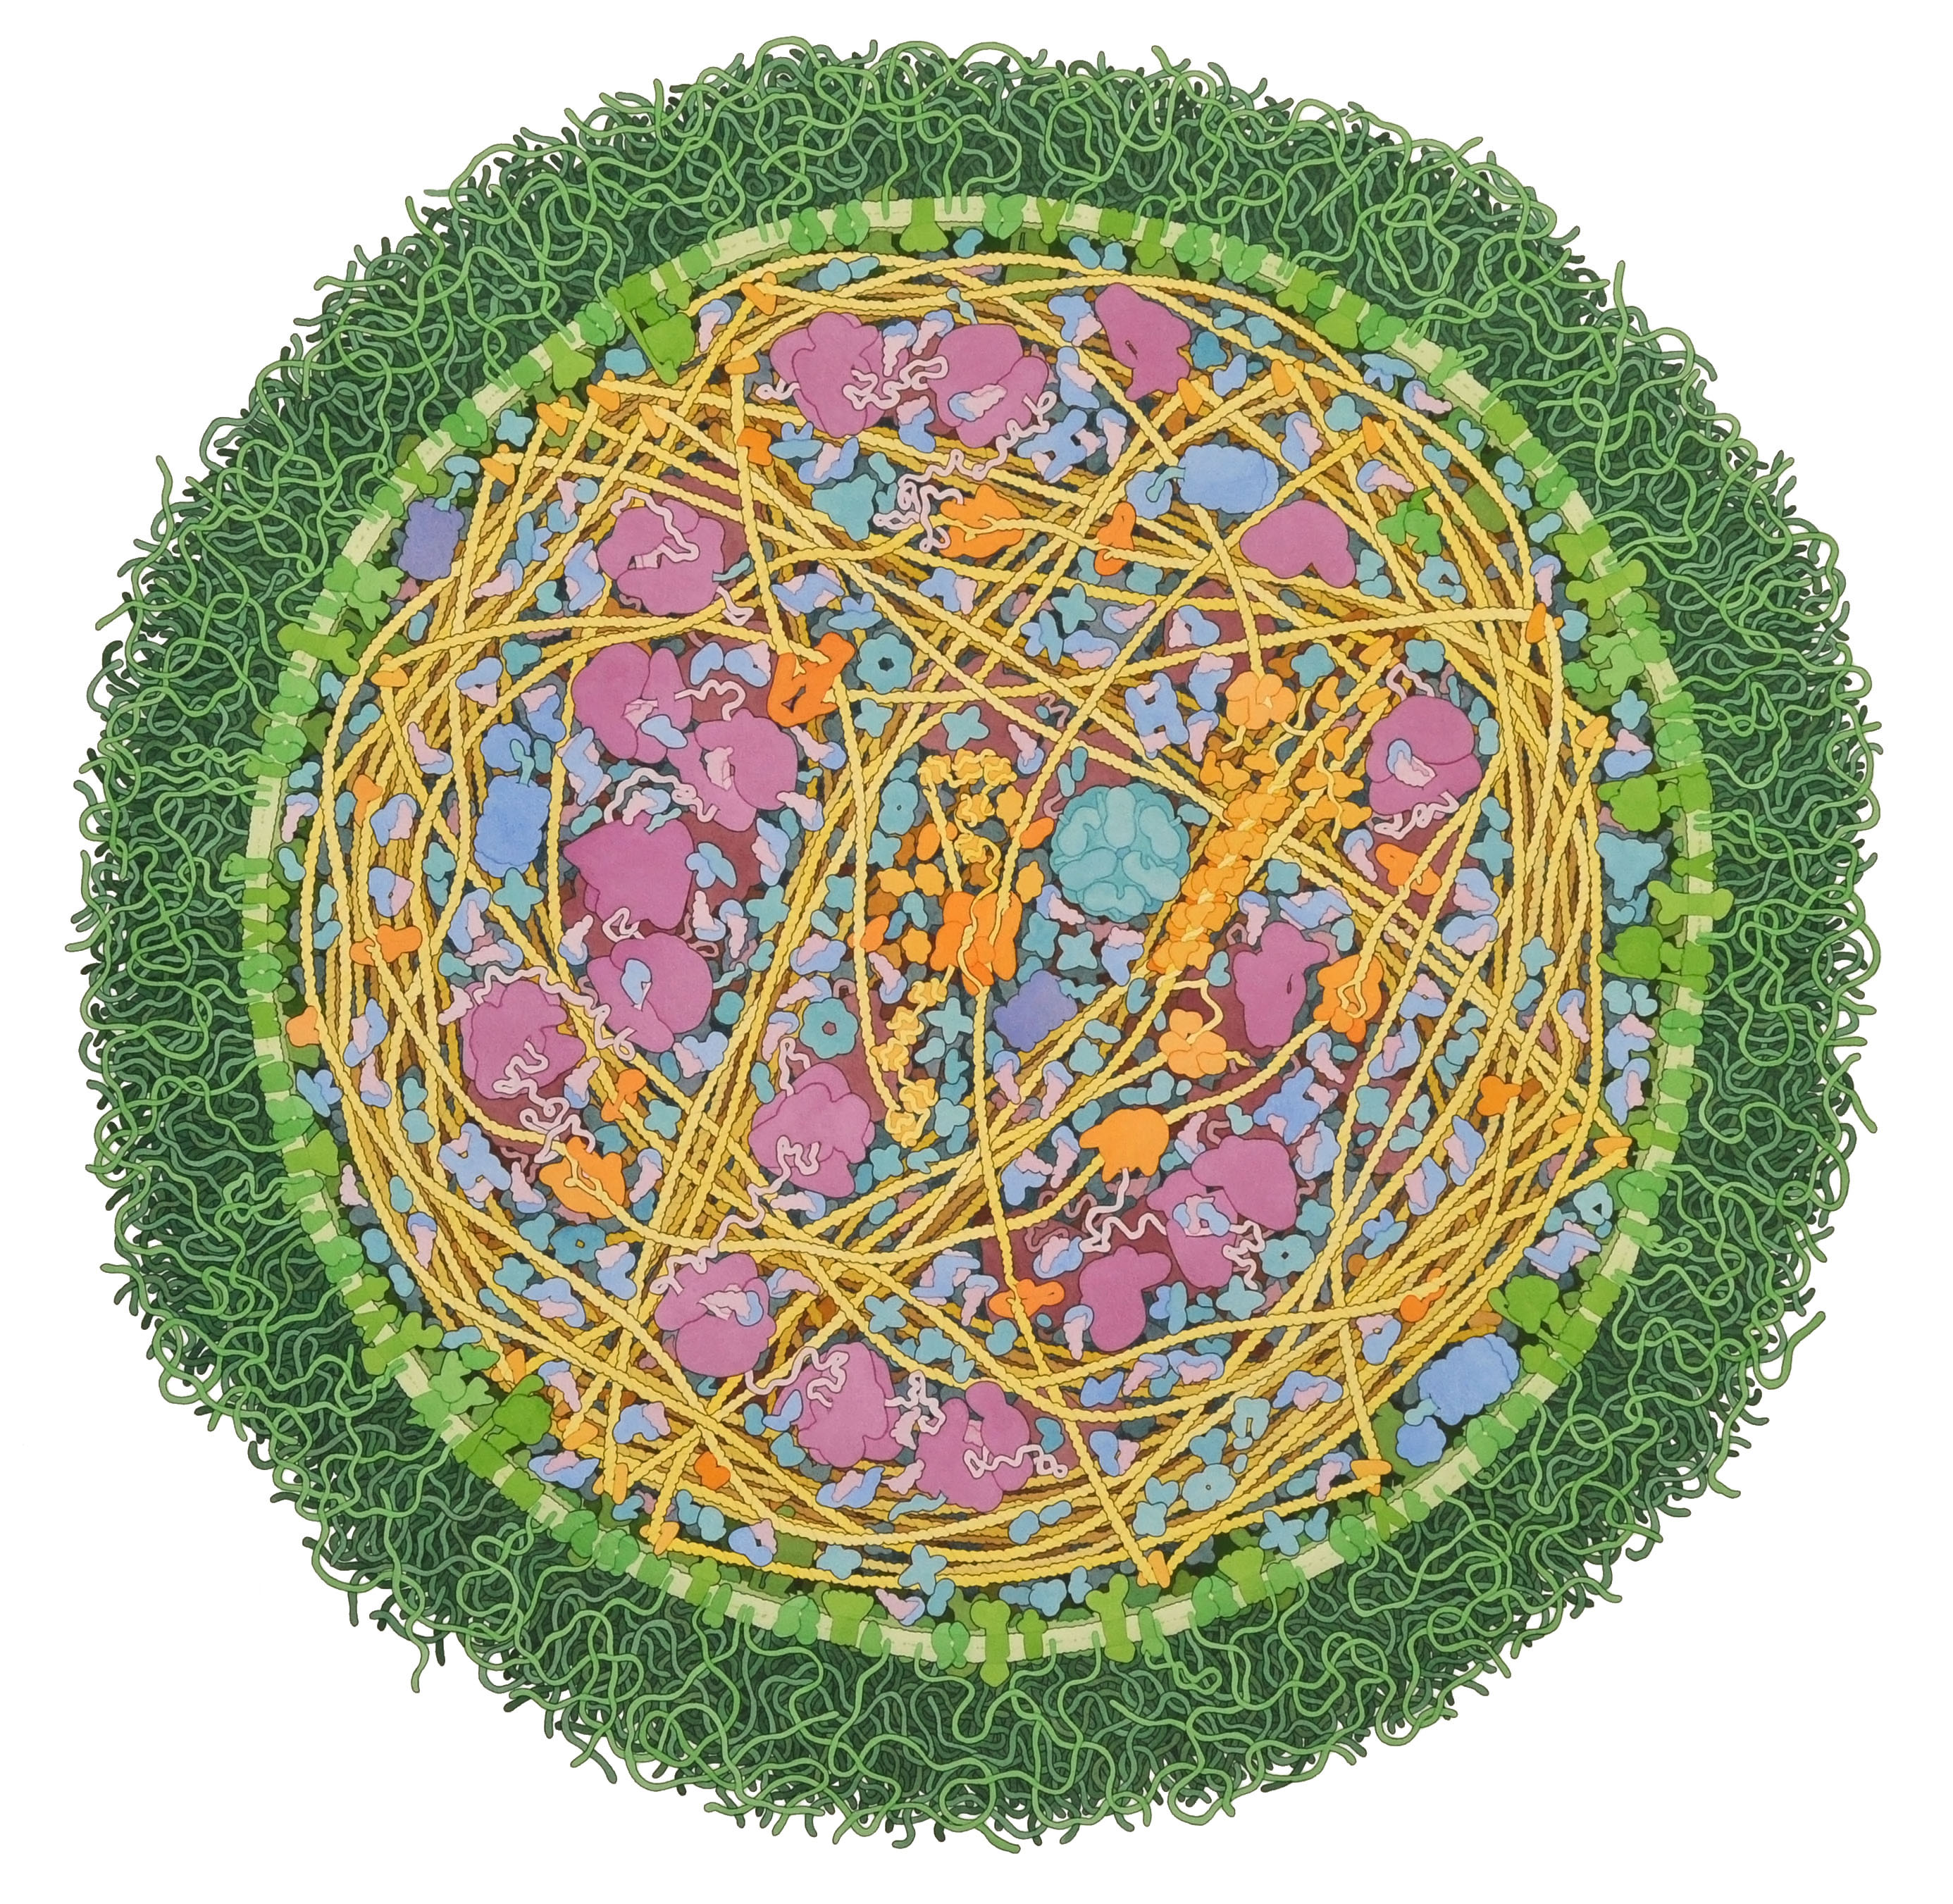
\includegraphics[scale=0.5]{images/goodsell-mycoplasma.jpg}
  \caption{David Goodsell's illustration of}
  \label{fig:goodsell-mycoplasma}
\end{figure}
% TODO: say that we are in domain of biological/molecular visualization
This thesis focuses on visualization of structure and function of objects in cell and molecular biology. To show examples of such visualizations we can point to works of Drew Berry \cite{DrewBerryMovies}, Graham Johnson \cite{GrahamCellVideo} or Janet Iwasa \cite{iwasa2010animating}.

% TODO: [\textbf{why are illustrations/animations useful: what art was talking about and also janet in molecular flipbook video}]
The importance of such work is not only in bringing the science to the laymen. Humans are visual beings and by seeing something we can understand certain concepts more deeply or differently. And this applies to other scientists as well. In practice this means that such artworks can serve as a discussion starters. New ideas, hypothesis and experiments might emerge just by seeing concepts differently or as a compilation of information into one cohesive artwork.

Scientific illustrators have to balance both the correctness and artistic form of their outputs. Where conventional artist can use visuals to supress or pick up his message, illustrator have only limited

There are many ways how scientific illustrators can do their job. Historically, illustrations have been done by hand with traditional drawing and painting methods. Even today, some illustrators still prefer this way of working. It is however a very timely process, as individual illustration can take months to make. Probably the most well known and accomplished person in this is David Goodsell\footnote{
  David Goodsell's web page: \url{http://mgl.scripps.edu/people/goodsell/}
}. Goodsell has developed a style of abstracting details while preserving the general shapes. However, this is a very timely process, as individual illustration can take months to make\cite{DavidGoodsellVideo}. If we consider the speed at which science is moving forward nowadays what could end up happening is that before an illustration is finished a new finding emerges, rendering the illustration effectively obsolete. This is of course undesirable and we need to look for ways how to accelerate, or even partially automate, this process.

% [\textbf{Can we use computer graphics for this?}]
With the increasing popularity of computer generated imagery, it has naturally been adopted by scientific illustrators as well. Tools have become more accessible and easier to use over the years. Today, software solutions like Maya, Cinemar4D or 3Ds Max have become industry standards for any task that revolves around modeling 3D geometry and rendering it. Game and movie industry are the leading industries that push computer graphics software creators forwards and provides most of the revenue for them. This means that these tools, no matter how versatile they try to be, are being skewed towards the use cases in movies and games. That means that people who want to create scientific content might struggle to use the tools sometimes. Still, people have been able create amazing images and movies showing people fenomena from all kind of science disciplines.

% before it was hard to make illustrations, now it's even harder because we want to do animations
With traditional methods it was timely to create just a static illustrations. This process can be sped up by using modern tools with the help of computers. But the bar has been raised by the need of animated concent and movies. Now this is what can take months to prepare. Using professional 3D tools certainly helps. For example, instead of frame-by-frame animation, physics simulations can be used to create animations which are (at least to a certain extent) physically correct. The problem that still persists though is that vendors do not design their products with a use in scientific illustration in mind. It would actually be impossible to do so when we take into account how much different uses we would like to employ this software. But we still need a way how to import scientific data into the program and work with them.

To do that, people have learned to customize this software\cite{GrahamGaelInterview}. Commercial 3D authoring software is by convention highly customizable via scripting and/or APIs. This allowed illustrators and animators to extend the software by implementing functionality that they need. For example, one task that commercial toolsets do not solve is loading scientific data and structures as models. Some of these have been released to public (as we will see in chapter State of the Art) but most of the scripts are being developed and used only by the original author.

% [\textbf{what are the alternatives to what people are using already?}]
From a completely different section of the field of molecular visualization, there are domain-specific tools.
There also exist programs that are completely separated from any of the mentioned commercial software. There is an active research in the domain of visualization, with many conferences every year and hundreds of research papers in this field comming out. Usually, as a byproduct, these paper generate software that showcases the proposed visualization technique or pipeline. Some of these have been turned into full featured visualization packages and thus provide a way how to illustrate something in a new way. While these programs might hugely benefit scientific illustrators, it's not always the case that they get used. This might be because of several reasons one of which is that the illustrators are simply used to a certain pipeline and incorporating a new software into this pipeline doesn't seems very beneficial to them. Another problem is that because these programs are developed for a certain use cases (showcasing the point of the paper) they might not be easily appliable to more than one purpose.

% [\textbf{``mission statement'' of the thesis}]
%In this thesis, we made an effort to solve these problems. Our domain of choice is molecular visualization.

%In this domain we try to visualize living (?) organisms on the smallest possible scale. With this approach, the computer memory and performance requirements are very challenging even for todays available hardware. Still, people have been able to visualize for example model of HIV in blood plasma in it's full detail down do individual atoms of each protein. This however, is achieved by using a very customized rendering method and a custom data format. In 3D graphics, data are usually represented as meshes consisting of triangles (which in turn are made of vertices). If we wanted to represent each atom as a sphere, we would need at least <number> of vertices for one atom and that's only for the roughest level-of-detail. With such representation, a one whole protein could use up to X bytes of memory which already takes up most of the video cards' memory. Thus this representation is not suitable for this task. Instead, various other techniques have been developed for rendering on molecular data.

%That being said, these techniques are not usually taken into account when 3D authoring software is developed. As was mentioned, the primary users of these software are video games and movies industry, where mesh representation is the one used. That implies that people that use these programs don't have access to the cutting edge technology of rendering, visualization and illustration of molecular data and there is room for us to improve this situation.

In the next chapter, we will describe the state-of-the-art programs and tools that are used for molecular visualization today and we will mainly focus on showing the gaps in intercompability of the available programs. Then, in chapter 3, we will propose a method of how the problem could be solved.

\chapter{State of the Art}
\label{chap:star}
%I think the sections could be: 3D Modeling Software (Maya, C4D), Niche (Specific) Tools (cellVIEW, ...), Data Generation (cellPack)
%Popsat: Molecular Flipbook, Molecular workbench, molecular maya, mcell, cellblender, pymol, VMD, ePMV(scripps)
Several approaches can be taken when creating an illustration, animation or interactive experience that has some basis in science. We will show tools that help with this process, describing its primary use, discuss its implementation and how this toold is or could be used. Listed solutions are the ones which we believe are or were pivotal or at least present ideas which we think are beneficial to this field.

First however, we will talk about the character of data that we are mostly working with in the field of molecular visualization.

%In this chapter we will introduce the software that is currently available for scientific illustrators working in molecular visualization. Illustrators have gone a long way from doing these works by hand and nowadays there exist a variety of programs that help them do their job communicating the scientific findings. However, as we will see there is are multiple level of user accessibility and different programs have different prerequisities on the level of expertise of its users. Given the fact that when communicating science one has to understand to a certain extent the science there are multiple ways to approach the design of the program. We also see that the

\section{Molecular Data}
All matter consists of \textbf{atoms} which are grouped in \textbf{molecules}. Atoms in turn contain protons, electron and neutrons which have their own internal structure. This is a level which is out of the scope of what is relevant to this thesis. Individual atoms are the smallest elements that we will consider.

\textbf{Biomolecules} is a term describing any molecule that takes part in some process in living organisms. \textbf{Macromolecules} are molecules that are very large, containing typically several thousands of atoms or more. We will not be dealing with chemical properties of molecules and therefore details like what forces hold which elements together are omitted. We are mostly interested in the structure of such objects-what they look like.

\textbf{Proteins} are macromolecules that are formed by a process called protein synthesis. During this process, part of DNA is transcribed into messenger RNA which is then turned into chain of amino acids that fold into a protein.

\textbf{Lipids} are hydrophobic molecules that typically serve as a building elements of lipid membranes. Lipid membranes separate different compartments in a cell.

% TODO: acquisition
Different techniques are used to acquire molecular data. The three most widely used are X-ray crystallography, nuclear magnetic resonance spectroscopy (NMR) and cryo-electron microscopy (cryo-EM). Each of these techniques has their benefits and downsides. For example, using NMR, only structures of limited size can be resolved. On the other hand, using cryo-electron microscopy can be used to resolve large structure but only in low resolution.

% TODO: pdb
RCSB Protein Data Bank is a database where the information about structure of large biological molecules resolved using these techniques is stored. Each molecule is identified by PDB ID, typically a four.... Data can be exported and downloaded in several formats, most notably PDB file format with extension .pdb. For us, the most relevant data that can be acquired from this file is the list of atoms with their XYZ coordinates.

% TODO: cellPACK
Between the molecular (observable with methods like NMR and X-ray crystallography) and cellular scale (observable with microscopy), there is an intermediate scale (mesoscale, 10-100nm). In general, there are no good method available to observe objects in mesoscale in atomic detail. Because of that models on this level must be compiled computationaly by using information from multiple sources. cellPACK\cite{cellPACK} is a software that does exactly that. With cellPACK we can assemble models of an intermediate scale by employing packing algorithms. A recipe serves as an input for this algorithm. A recipe is a compilation of data from light and electron microscopy, x-ray crystalography, NMR spectroscopy and other biochemical data. The process then has two steps: gathering of the data to compile a recipe and then assembling a virtual model from this recipe. cellPACK has been developed at Scripps institute and is a biological version of a more general software called autoPACK. Both of these are implemented in Python and open-sourced.

%\section{Commercial 3D Software}
\section{Professional 3D Software}
% [\textbf{Commercial 3D software is absolutely dominating}]
Using a professional 3D modeling and animation software can help scientists to communicate their ideas. These programs have been designed to provide means for people that need to create three dimensional models of any kind. And in the past several years, more and more scientists do employ professional 3D solutions into their pipeline for various purposes.

Unfortunately, these programs usually come with a very steep learning curve. Mastering this tool, or even getting on proficiency level enough to produce meaningful work, is not an easy task and takes between several months to years. This is not something a lot of researchers are willing, or even able, to sacrifice. The good news is that there is usually a number of learning materials available on the internet, both supplied by the vendor of the software and third parties.

Another problem with software meant to general 3D editing is that these tools are not designed with molecular visualizations in mind. This is problematic because of the fact that scientific illustrators want to work from accurate data. Mentioned software is primarily designed to be used by workers in entertainment industry. Thus there is missing any framework which would enable to import scientifically accurate data in the basic program installation.

There is number of options to choose from currently available products. Most widely used are Autodesk Maya and Cinema 4D although other programs have been successfuly used in various projects. We can name open-source Blender or a relatively young product MODO\cite{MODOscientificIll}.

%[\textbf{things that are nice to have from these programs - easy manipulation with objects, scene graph to organize the scene, tools for animation, semi-automatic object positioning (random, particles)}]
Disregarding the differences between all the 3D software of this kind, there are features that are more or less contained in all of them and over the years have become must-have features that tremendously help with navigating and editing of 3D scene.

First, objects in scenes are organised into some variation of ``scene hierarchy'' or ``scene tree''. This allows users to organise their objects and establish parent-child relationships between these objects.

Second, navigation in the 3D scene is always solved to be intuitive enough to provide efficient ways how user can position his view. Every named program allows the user to open multiple viewports at the same time where every viewport shows different camera position.

Third, object manipulation—translation, rotation and scale—is solved and made available under shortcut which allows the user to work efficiently. Shortcuts are often instruments each individual artist gets used to and might have a hard time switching to different product.
% TODO: images: scene hierarchy across the programs: maya, c4d, blender?
% TODO: images: object manipulation
%These are the killer features and even though they are present in all of the programs, the illustrators are often used to the way they work or to a certain shortcut which means that it's not trivial for them to switch from one to another (or it is but it takes some time).

% TODO: rendering

%[\textbf{scientists have to go through training to be able to use these programs}]
%However, as we said in the introduction, by having the information compiled into visual form is hugely beneficial so some people were willing to dive into learning these tools and have been able to use them to an incredible benefit. Ideally we would like more scientists to be able to create visuals like this so attempts to simplify this process have been made.
Despise the mentioned drawbacks, professional 3D software is being widely adopted as a solid base of workflow of scientific illustrators and animators. Once illustrators overcome the initial learning period, general 3D software becomes a powerful tool in their toolset. 

\subsection{Plugins}
%[\textbf{We have an ``entry point'' which we can exploit to inject our custom functionality}]
It has become a convention that all of the professional 3D authoring packages (like Maya, Cinema4D or even Blender) provide one or more means how users can program additional functionality. There are two major ways how vendors accomplish this.

First, scripting interface is provided. This means that user can both perform operation and trigger actions by using GUI but in addition to that they can do the same (and in most cases even more) by calling particular commands via a command-line-like interface. Obviously the capability of these additional implmentation is limited and scripting interface is mostly used to automate tasks which would otherwise take too much time.

Second way is the ability to load plugins that use Application Programming Interface, or API, designed by the vendor. API provides classes and functions that can access and alter internal state of the program or the data inside it. This way the user can implement functionality that he or she is missing from the basic program. Thanks to that these 3D authoring programs can be adapted to more specific use cases.

%[\textbf{Tools where people already used this plugin architecture}]
Some of these plugins have actually already been implemented to help artists in molecular illustration. The most prominent is Molecular Maya which, as the name suggests, extends Maya with the ability load and manipulate models of macromolecules from Protein Database. Molecular Maya plugin gives its users the ability to load macromolecules based on its PDB ID or locally from pdb file. After the model is loaded, user is able to select the display representation (between TODO: vyjmenovat) and also select with how much detail the model should be rendered. Molecular Maya plugin is free with the option to purchase upgraded version which provides more advanced functionality.

BioBlender

Similar plugin exists for Blender modeling program as well. It's name is cellblender
% TODO: bioblender: http://www.bioblender.eu/

%[\textbf{How people normally render - offline}]
The rendering stage takes place after the scene is modelled. Again, there are more options at hand. 3D packages usually come with a default rendering solution which is for the most part good enough to use. For more demanding artist, external renderers like vray, mental ray, corona or octane. What these renderes have in common is that they are so called ``offline renderers''. In practice this means that they are using ray tracing (or similar) technique to render the scene with a process that is very much close to how light works in real life. The disadvantage of this approach is that this process take more time. It usually isn't possible to achieve real-time rendering (fps at least 25).

%[\textbf{interactive renderers like octane, how do they fit and why they are not the full solution}]
%In recent years, interactive renderers have been gaining popularity. These tools work in a similar way as did previously offline renderers. The difference is that they show the artist an intermediate result of the path tracing (or the technique they are using). This way the artist gets a fast render of his scene with a lower quality and the quality of this image is refined iteratively. This approach also enable its user to see changes in the scene in a quick preview and as it is right now, a lot of artist have been using this feature and they say it's been greatly helping them in their work. There is however one thing that we can still improve. These renderers still operate on meshes. We've already talked about how our data can be efficiently simplified to our purpose and therefore rendered with a great performance in real-time. Thus even if interactive renderers like Octane could improve the workflow we can still provide a better performance by using custom renderer like cellVIEW.

\section{Domain-specific tools}
%kinemage (http://kinemage.biochem.duke.edu/), chimera (http://www.cgl.ucsf.edu/chimera/), jmol?
%[\textbf{intro}]
In the field of molecular visualization as a research topic, numerous programs exist. They share a lot of features but they each have their own specialities and are meant to be used for slightly different tasks. We will name a few that have been developed for some time and have matured to a certain extent. Apart from that, other tools exist which are even more specialized. These might be results of a research and they accompany a paper describing the technique. This means that these programs are not that well usable out-of-the-box but rather serve as a demonstration of a certain technique.

%\textbf{Molecular Flipbook}
One of the more user-friendlier and easier to use tools is \textbf{Molecular Flipbook}. It has been develoved by a team lead by Janet Iwasa and it consists of two parts - an animation program and a website where creators can share their works. The main motivation for this project is to create tool that even scientists without education in animation can use to communicate their ideas through simple molecular animations. They achieve this by building the program around the concept of simplified key-frame animation technique. The website portion of the project is meant to serve as a database of animations explaining various processes. Creators can upload their works and improve works of others.
%[\textbf{TODO:} cons, done on top of a blender game engine, info: http://mikepan.com/flipbook.html]

\textbf{Molecular Workbench}?

\textbf{PyMol}\cite{PyMOL} is a more mature project which aims to be used by more expert users. It is an open-source software product in which the user can view, render, animate and export 3D molecular structures. PyMOL can visualize molecules with several representations - spheres, surface, mesh, lines, sticks, etc. Rendering can be done with internal ray caster. Based on Python.

\textbf{VMD} (Visual Molecular Dynamics)\cite{HUMP96} serves as a tool for modeling, visualization and analysis. It actually has a long tradition, bening first introduced in 1996.

\textbf{cellVIEW}\cite{cellVIEW_2015} is a tool with the ability to render large biological macromolecular scene at an interactive frame-rate. It has been designed and implemented with regards to this use case with the use of state-of-the-art rendering techniques. It employs several modern techniques to reduce the amount of processed geometry in macromolecular scenes to provide its users with a real-time performance. As a result cellVIEW can render scenes containing up to several billion atoms with a framerate above 60 fps (?). cellVIEW has been implemented with Unity game engine. The rendering styles has been inspired by illustration by David Goodsell who has developed a style of abstracting the shape of individual proteins to reduce visual noise of the picture. cellVIEW immitates this approach by integrating a level-of-details scheme - the farther the protein is from the camera the less amount of its atoms are rendered and the rendered atoms are scaled up. This approach results in a multiscale visualization - user can zoom in to see individual atoms of a protein instance, or he can zoom out and see the whole dataset with its distinguisable compartments. The biggest dataset that has been possible to visualize is HIV, however tests have been done and it should be possible to render e-coli bacteria (which is X times larger)

ePMV tackles similar problem as we do. The goal is to simplify process of generating figures and animations for scientific purposes. ePMV is a plugin which brings molecular visualization toolset into various 3D authoring software. It is using the plugin-using-API architecture which most of the programs provide to implement an unified environment for the molecular tool to run on. 
\textbf{ePMV}\cite{ePMV} is a project that has tried to solve a similar problem as we do. ePMV is a system which brings molecular visualization toolset into various 3D authoring software. It's building upon the plugin/API architecture which most of the programs provide. They implement an adaptor module which is a plugin for each of the supported 3D programs. This adaptor provides an interface for the actual molecular software to run inside the host 3D program. Uses uPy. We don't use Python.

\section{Workflow}
% [\textbf{Define the workflow - how it is now and how we could improve it (fasten it)}]
The actual workflow obviously differs from illustrator to illustrator, different software is used, different plugins and most importantly different data and project goals.

It is however important to formalize a little bit how the workflow looks like. Our goal is to connect one of the specific domain tools into a professional software. By doing that, we want to achieve faster and therefore more effective workflow.

In general the pipeline is composed of two major steps - modeling and rendering. In the modeling step, all the data, requirements, hypothesis, ideas and stories are compiled into a 3D scene or animation. Artist usually uses software-specific features like particle systems, physics simulations,... to get there.

The next step is generation of either still image or animated video from the 3D scene/animation. This is equally, maybe even more so, important as the first step. By using certain rendering techniques we can underline concepts which are important to the artwork. The level of . Traditionally, this step has been very computationally intensive. Today with the power of modern GPU and the increasing availability of such devices, the render times have been reduced to X-Y. Still, this represents an obstacle in the workflow of animator.

% yeah it's good to end this with workflow because I can talk here about how things are and what is the problem that we want to solve and in method I can continue with that and it's exactly as we talked with Ivan about the Problem definition
This is the problem that we wanted to solve by using custom state-of-the-art molecular renderer. As was mentioned before, at this domain, the super-realistic results of modern rendering methods are not beneficial to us. We instead want to employ more illustrative, simplified rendering style. That brings us another benefit in that this rendering method is better performing allowing us to render at interactive (real-time) framerate. By using our fast renderer, we want to eliminate the time cost of rendering step when using conventional offline renderers.

\chapter{Method}
\label{chap:method}
%[image: modeler, renderer, illustrate the connection through shared memory, data streaming, camera position]

%[\textbf{we focus on fastening the workflow by using our renderer}]
As was discussed in State of the Art chapter, the majority of artists uses commercial 3D software. These programs are very good at modeling and rendering 3D content as a set of meshes - 3D objects consisting of triangles. However, for molecular data and scenes, mesh is not the best representation and there exist rendering techniques that perform way better if we use other representation.

%[\textbf{we can take advantage} of the fact that illustrators use illustrative style, simplified and the data is very compact actually so we can provide them the interactive preview]
Another thing we can take advantage of is that illustrations and animation describing structures and function of objects at nano-scale don't often profit from using ultra-realistic rendering. The concept of realistic rendering and light/material interactions don't exist at this scale. They show concepts that are happening at different scales than the stuff that programs are usually made for. Thus they usually want to use more illustrative, simplified, rendering styles.

In our use case, this is even more true because we are dealing with a very dense data sets. We want to simplify what we show to reduce the visual noise in the ouput image. Various level-of-detail (LOD) schemes exist and they not only help with filtering of the visual noise but also reduce the performance requierements.

Thanks to these simplifications we can render molecular scenes with interactive framerates, as has been shown by cellVIEW\cite{cellVIEW_2015}. Unfortunately, these techniques are not implemented in 3D commercial programs which is what the artists usually use. Our goal is to make it so that the artist can use his software of choice to model his scenes but also take advantage of modern rendering. The use is two-fold: real-time rendering can serve as a preview of the scene but also can be used as a final result. The goal of this project was to come up with an idea of how to connect these two programs so that they will work together.

\begin{figure}
  \centering
  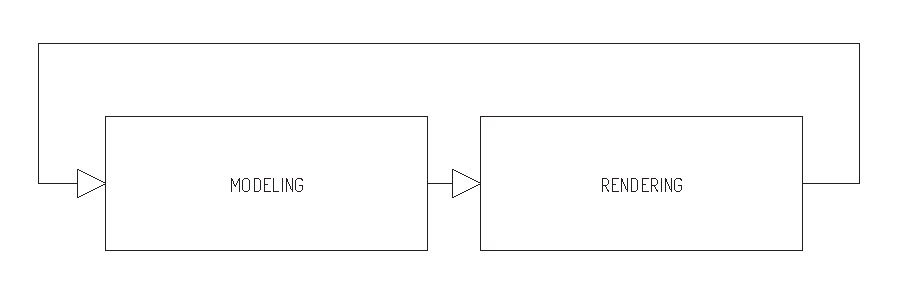
\includegraphics[scale=0.8]{images/pipeline.pdf}
  \caption{workflow}
  \label{fig:workflow}
\end{figure}

%[\textbf{two options, we choose third}]
Ultimately, we have two programs and we want to use some functionality from the first one and other functionality from the second one. The naive solution would be to implement our desired functionality into the software that is missing it. In our case, that would mean we could either implement the fast and visually appealing rendering into our modeling software, or we could do the opposite and implement the desired modeling tools into our renderer.

The problem with the first option is that most of the 3D software packages that artists are using the most are commercial solutions with closed source code. It is possible to extend them via API that they usually provide but that is not enough if we want to implement state-of-the-art technique that sometimes requires the latest technology in terms of graphics API etc.

We've chosen to go with another, third, option. We don't want to reimplement from scratch something that is already available to use. We want to avoid this development overhead. Instead, we went for a different approach and tried to connect the two parts in a way that would allow us to use both features at the same time. We do this by using both of the programs and establishing a communication channel between them. We use writing and reading from shared memory to accomplish this communication. In our case the communication is one-way. We have a modeled scene on one side and we want to transfer data describing this scene to have it rendered on the other side. As we will show this can be done in a straight-forward fashion as our scenes can be simplified to the point when we can describe them with few numbers.

%[\textbf{why is it that we can do this?}]
We can establish such communication between the two programs mainly thanks to the character of the data we are dealing with.

%[\textbf{the data}]
Scenes we work with consist of macromolecules - proteins and lipids. Macromolecules in turn are made of atoms of different elements. There are multiple representations by which we usually visualize atomic data (see chapter State of the Art) [TODO: where should I put this?]. However the underlining data doesn't change. An instance of molecule is defined by the type information (what kind of molecule this is), position and rotation of the instance, and last, a list of atoms that this molecule is made of.

% we will use some placeholder geometry in maya
On the side of modeling program, we want to see an approximation of the scene. One way would be to use a simple geometry like cube or sphere as a placeholder for each molecule. Such placeholder would then serve as an object that we manipulate instead of an actual molecule. We tried something a little bit different. With Molecular Maya plugin, we can load a molecule description in form of a pdb file. With the same plugin it is also possible to generate a polygonial surface mesh representation with choosable detail level. We therefore load a molecule and generate very low resolution mesh which serves as our placeholder.
% TODO: IMG: show low poly model of a protein generated with mol maya

%[\textbf{overview of the method: two ends, shared memory, what needs to be transfered, ...}]
On the Figure X, you can see an overview of the system. On one side we have a modeling software while on the other we have a domain-specific tool, in our case it's a high performance renderer. Our vision was to have both of these programs running at the same time. The illustrator could have his scene opened in his modelling software. This way he would be using the tools he knows and is accustomed to for modelling the actual scene. Then on the renderer side he would be able to see how the changes he's made are reflected in the rendered final image. This all would happen in real-time thanks to writes and reads into and from shared memory.

% [\textbf{simplifications, how the scene can be described}]
As was already mentioned, when dealing with molecular data we can take advantage of several simplifications. A scene like this consists of macromolecules: proteins and lipids. First simplification - we consider the shape of the molecule to be static. This means that inside each molecule, the positions of all the atoms doesn't change in time. The position of the atoms is taken from the PDB file. The second simplification is that all the instances of certain molecule type look the same. They only differ in position and rotation.

% [\textbf{what data do we need to transfer}]
With these facts in mind, we can define a molecular scene as a set of molecules, where each molecule is defined by its position, rotation, and type, which says what kind of molecule this instance is.

This means that we need to stream this data - positions, rotations and types - of all molecule instances from the modeling software to the rendering tool. Because of the technical implications we write the data in a format described on Figure X. This is more efficient that writing the data in a format position/rotation/into for each molecule.
\section{Process}
\subsection{Parsing the Scene}
% [\textbf{the actual process}]
Inside the modeling software, we scan the scene, looking for molecular objects. We need to identify an object which is supposed to represent an instance of a molecule. We find out what type of molecule this is. This information is saved in a form of pdb id. For each of the found instances we also read its world position and rotation. This info is accumulated into an array and then prepared to be written into the memory.

There are several approaches and optimizations possible at this level and these depent mostly on the API that the modeling software provides. We were able to inject this method into a callback which is called everytime a scene has changed. After this happens, we scan all the models in the scene and look for molecular objects. This could be optimized in a way that only the objects that have changed report their changes. That way not all the object in the scene need to be scanned which saves us some performance. As we've discovered however, the APIs are not always keen on having such a performance-heavy procedures executed on each frame and so the concrete implementation heavily depends on the chosen modeling software and its API. We will describe in more detail how we accomplished this with Maya API in the chapter Implementation.

\subsection{Writing into and Reading from Shared Memory}
Once the data about current state of the scene is accumulated into position, rotation and info arrays, we can write these into the shared memory. Operating system api calls should be used for this. Again, for more details, see chapter Implementation to see how we did this on Windows operating system.

\subsection{Using the data}
Reading the data uses operating system api calls as well. In our case, because we are operating on the interface between c++ and c\#, the code that reads from the memory is pretty simple, only retrieving memory address and sending it into the c\# part of the system. This data is then copied into buffers inside cellVIEW which in turn sends them to GPU for render. We format the data in a way so that there is no additional manipulation on the data between these steps required. After the data write, we ideally want to only copy the chunks of memory from one place to another.

%[\textbf{Why Maya?}]
We have chosen Maya as the modeling software because our collaborating partner, Drew Berry, is its prominent user and he's been a key person that we had in mind when implementing this method. Chosing cellVIEW as the renderer has been an obvious choice as its rendering capabilities are on the state-of-the-art level of what common hardware computers are able to render. Drew Berry has been impressed with the results of cellVIEW and expressed his interest in using it for his movies.

\section{old}

[\textbf{we don't want to use files} TODO: why?]Our method tries to solve these two problems. The problem of import/export is solved by using shared memory instead of files managed by the user. The rendering times problem is solved by using modern rendering techniques which enable us to render what we want in an interactive framerate.
The reason why it's possible to take this approach of using shared memory comes from the character of data that we work with. Molecular scenes consist of molecules. Molecules are made of atoms which can be, and usually are, represented as spheres. Atoms of different elements are visualized by having different radii and colors. So for every molecule we need to keep track of what atoms it consists of, positions of those atoms and type of each of those atoms. This is even more leveraged by Protein Data Bank, which stores data about various proteins that have been found through out the years. For us, this means that we only need to keep track of the type of molecule and by fetching data from Protein Data Bank we get information about the protein cataloged under the protein identifier. Our scenes are (simplified) made of macromolecules. That means that in the end for rendering the scene we need a list of molecules, where for each molecule instance we need to save it's position, rotation and type. That's all the info that we need to be able to render our large molecular scenes. Even though this is still a lot of data, we are slowly getting to being able to render this on commonly available hardware. Because of the fact that this data size is "manageable" by modern computers we are able to store the data in shared memory.
This method is mostly valuable as an example of how interconnection of software can be done and what improvements to the users this can bring. There is some prerequisities - both programs need to be extensible to the extend of the programmers must be able to develop extension that are able to read from and write to the shared memory using operating system api calls.

\chapter{Implementation}
\label{chap:implementation}
%Outline:
%[\textbf{high-level overview}]
%[\textbf{maya side plugin}]
%[\textbf{unity side plugin}]
%[\textbf{unity side c++/c\# interoperability}]
%[\textbf{unity side script - how the data is used/rendered}]

This chapter will in detail describe the implementation of real-time scene data sharing between Autodesk Maya and cellVIEW. Autodesk provides Maya users an API which allowed us to extend this program with required functionality. Similarly, we have been able to create plugin for cellVIEW. This was because of the fact that cellVIEW is implemented using Unity engine which also allows custom plugins in a form of DLL to be used.

\begin{figure}
  \begin{center}
    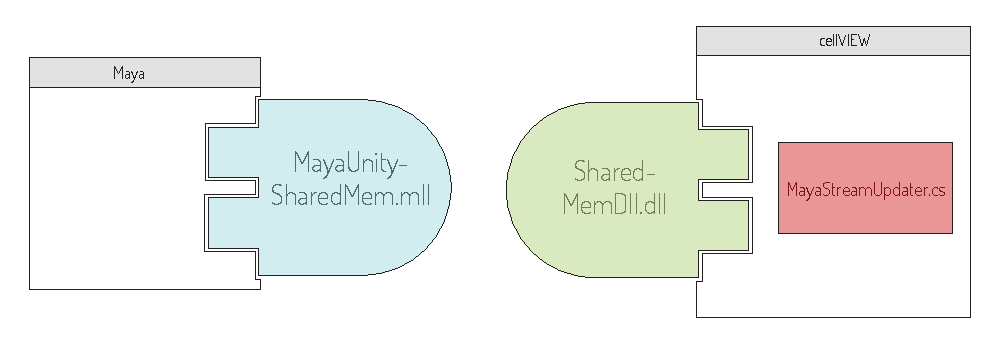
\includegraphics[scale=0.8]{images/system-architecture-overview.pdf}
  \end{center}
  \caption{Overview of system components}
  \label{fig:system-overview}
\end{figure}

% [\textbf{high-level overview of the architecture}]
The architecture of the system consists of three parts - a plugin for Maya, plugin for Unity and a Unity script - as you can see in Figure \ref{fig:system-overview}.
The data flows only in one way - we write into shared memory with Maya plugin and read from shared memory with Unity plugin. This simplifies the situation from the implementation point of view because we don't have to design synchronization scheme.
The plugin for Maya is using Maya API (which will be described later) and is written using in C++ programming language. The function of this plugin is to parse the 3D scene, looking for a molecular objects, and output their positions and rotations (along with info about the instance) into the shared memory.
Unity side of the system consists of two parts - a C++ plugin and a C\# script. The C++ plugin takes care of reading the data from shared memory, while the C\# script, which is a part of cellVIEW, receives this data and uses them to render the final molecular scene. Note that there are two types of interoperability between components: (1) shared memory functionality, which enables two processes to communicate, and (2) interoperability between C++ and C\#, which allows us to pass memory addresses from the plugin to the script on Unity side.

% [\textbf{shared memory} - talk general about shared memory technology]
\section{Shared Memory}
Shared memory is a segment of system memory which can be accessed by multiple programs. It is used as an efficient way to establish communication between separately running processes. Our implementation has been done on Windows, however the concept of shared memory can be found on all operating systems.

% TODO: swaping onto disk, unix, named file mapping in windows
From now on, we will be talking about the implementation that has been done on Windows operating system. There are several way how we can access shared memory here. boost library provides class that provides an abstraction above shared memory functionality. Similarly, Qt framework also has class with comparable function set. We chose to not use any of these. Instead, we directly used Windows API function calls to operate with shared memory. This solution has been chosen because we wanted to use the lowest possible layer because of speed concerns. This unfortunately means that our implementation is tied to Windows platform. Porting to other platforms should however be straight-forward.

\section{C++ and C\# interoperability}

% [\textbf{maya api}]
\section{Maya API}
Maya actually provides two APIs - one in Python \cite{MayaAPIPython} and one in C++ \cite{MayaAPICpp}. In addition to that, there is also third way how additional functionality can be implemented - MEL scripting language \cite{MayaMEL}.

% TODO: talk about plugin types: command, node
% TODo: talk about typlessness

\subsection{MEL vs. Python vs. C++ in Maya}
MEL (Maya Embedded Language) is very similar to other scripting languages like Bash or Perl. It is not fully mature programming language and therefore is suitable only for things like automating tasks that would otherwise be done through the GUI. There is however one thing in which MEL excells and is perfectly suited for inside Maya programming ecosystem - creation of custom GUI. Even though graphics interface can be made by using modified Qt library \cite{MayaQt}, extending the interface is way faster and easier with MEL.

Python API is more mature then MEL. Its advantage is that Python, as an interpreted language, can be run without compilation. This means that there doesn't have to be a compilation step and this makes the iteration loop faster. However, Python is, naturaly, expected to be slower than C++. We wanted to implement a functionality that is real-time. This means that we needed every piece of performance we could get. Because of that, the C++ API has been chosen and thus our Maya plugin has been implemented in C++.

There is also another reason why only the C++ route could be taken. We wanted to write into shared memory. The most basic way how to do that is via system API function calls. In our case, we implemented this on Windows platform. Thus the API we used has been WinAPI.

\subsection{Dependency Graph}
Maya's internal scene representation is called Dependency Graph. It is a network of nodes where each node has a set of inputs and outputs. Through these inputs and outputs the nodes are connected and data is propagated through the network. The idea is that each node performs some computation using input parameters and forwards the result further. There is an optimization in this approach in that the calculation is only done when the input parameters have changed somehow. If an output of a node is requested when the inputs have not changed, instead of performing the computation, a cached value is returned.

\subsection{DAG Hierarchy}
DAG (Directed Acyclic Graph), as the name suggests, is a structure in which nodes are connected with edges that have an orientation with the constraint that they can't create loops. In Maya API context this refers to a hierarchy of nodes which establishes parent-child relationships between them.
% TODO: illustrate with transform -> mesh so that I can reference to it in Maya side section

\subsection{Wrappers, Objects, Function Sets and Proxies}
In Maya API, we can find four types of C++ objects: wrappers, objects, function sets and proxies.

\textbf{Wrapper} objects usually provide utility functionality either for easier manipulation with data or mathematics. These include classes like MFloatArray, MMatrix, MVector, MQuaternion or iterators for traversing collections of data - MItDependencyGraph, MItMesh...

\textbf{Objects} and \textbf{Function Sets} are used to access and change internal object in Maya. Objects are instances of class MObject and they basically serve as a handle which only holds the necessary information about kind of object do they point to. In a way Objects are typeless and their type is determined by a mechanism called RTTI (Run Time Type Identification). Function Sets are here to actually perform operations on Objects. Function Set classes always start with a MFn* prefix and they are designed to be compatible with only certain Objects.

\textbf{Proxies} are classes that allow developers to implement new types of objects like custom nodes or commands. Proxy classes are always prefixed with MPx*.

\section{Maya side}
\begin{figure}
  \centering
  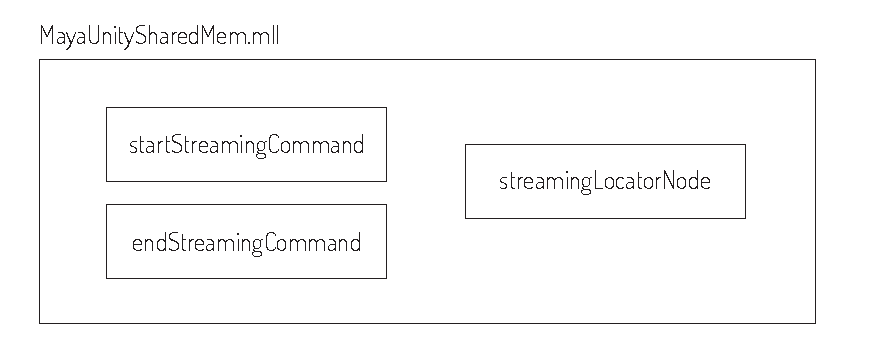
\includegraphics[scale=0.8]{images/plugin-contents.pdf}
  \caption{Plugin contents}
  \label{fig:plugin-content}
\end{figure}
%Topics - Architecture of the plugin, what parts/classes of API are used, memory layout, what I tried and didn't work.
Maya plugin implements two new custom commands and one new custom node. When the plugin is loaded and initialized it creates a new menu item in Maya's main toolbar. Under this menu item there are two subitems (buttons) - Start Streaming and Stop Streaming. These are set up to trigger call of appropriate command - startStreamingCommand to start the streaming and endStreamingCommand to stop it. This interface is made to adapt to the state of streaming, you should not be allowed to stop streaming when no streaming is happening and you shouldn't be able to start streaming when you already are.

The new custom node is class which inherits from MPxLocatorNode. This is a proxy type objects (as can be told from MPx prefix) and it serves as way to implement new node type. In this case the node is a locator node. What this inside Maya means is that handle that you use when you change objects in maya scene. This doesn't really sound like something we are trying to do. And indeed this is a little bit of a hack. We needed to implement our functionality in a place in Maya APi that would be called every frame, everytime something in the scene has changed. MPxLocatorNode has a method draw which can be overriden and this way we can implement our custom functionality which will be performed everytime something in the scene changes.

Another option would be to use connection of inputs and outputs and perform the code when these changes happen.

startStreamingCommand adds an instance of the custom node into the scene. 

% TODO: mention legacy viewport usage
% TODO: MPxLocatorNode

% TODO: left/right handed conversion
% TODO: image: new menu item
\section{Unity side}
On the side of cellVIEW (or Unity), we have two components - dll plugin and a C\# script.
Topics - Architecture of the plugin, very generally about plugins (it's just a basic C++ dll plugin), interface between C++ and C\#

\chapter{Demonstration}
In this chapter we present two use cases of how the user can approach illustration with this new proposed system.
Use case one - modified Janet's scene.
Use case two - microtubulus (create a model in maya and then name it properly and we will get it in cellVIEW).

\chapter{Discussion, future work}
The strongest use of the tool as of right now is the live preview of the scene. 

Limitations (of the tool) - what was done just for the use case and should be worked on for final production.
The project has been presented to Drew Berry (I think). Also, it was mention in a talk in Utah, presentation by Peter Mindek.
The method has tremendous potential in its application. The current implementation should be extended for both performance and actual use for artists. For this however, we will need additional input from domain experts. We have been fortunate enough that Drew Berry really liked this work and expressed his desire to develop this project further. It is highly probable that we will be working even more closely with him and that we would continue to improve this system so that he can use it for his movies production.
The challenge will be how to design the system to be easily adaptable by other creators as well.


\newpage
\printbibliography[heading=bibintoc]

\appendix %% Start the appendices.
\chapter{Appendix}
Here you can insert the appendices of your thesis.

\end{document}
